\chapter*{Proposition 44}



\begin{figure*}[ht]
    \begin{center}
    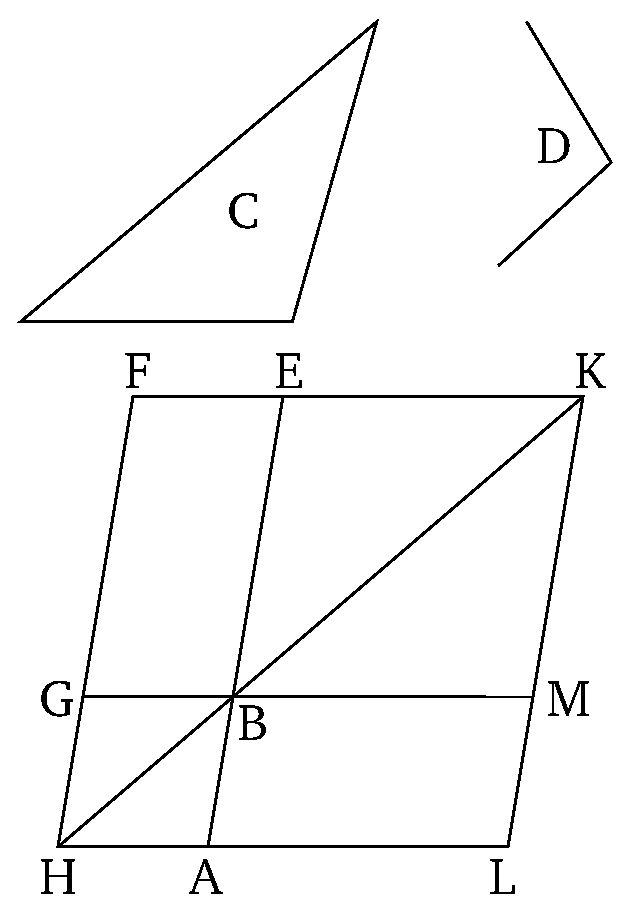
\includegraphics[width=0.5\linewidth]{figures/fig44e.eps}
    \label{fig:prop_44}
    \end{center}
\end{figure*}

To apply a parallelogram equal to a given triangle to a given straight-line
in a given rectilinear angle.\\

Let $AB$ be the given straight-line,  $C$ the given triangle, and $D$ the
given rectilinear angle. So it is required to apply a parallelogram
equal to the given triangle $C$ to the given straight-line $AB$ in an angle equal to (angle) $D$.

Let the parallelogram $BEFG$, equal to the triangle $C$, have been
constructed in the angle $EBG$, which is equal to $D$ [Prop.~1.42].
And let it have been placed so that $BE$ is straight-on to $AB$.$^\dag$  And
let $FG$ have been drawn through to $H$, and let $AH$ have been
drawn through A parallel to either of $BG$ or $EF$ [Prop.~1.31], and
let $HB$ have been joined. And since the straight-line $HF$ falls across the
parallels $AH$ and $EF$, the (sum of the) angles $AHF$ and $HFE$ is thus equal to
two right-angles [Prop.~1.29]. Thus, (the sum of) $BHG$ and $GFE$ is less than two
right-angles.
And (straight-lines) produced to
infinity from (internal angles whose sum is) less than two right-angles meet together [Post.~\ref{post:5}].
Thus, being produced, $HB$ and $FE$ will meet together. Let them have
been produced, and let them meet together at $K$. And let $KL$ have been
drawn through point $K$ parallel to either of $EA$ or $FH$ [Prop.~1.31]. And
let $HA$ and $GB$ have been produced to points $L$ and $M$ (respectively). Thus, $HLKF$ is a parallelogram, and $HK$ its diagonal. And $AG$ and $ME$ (are) parallelograms, and $LB$ and $BF$ the so-called complements, about $HK$. Thus, $LB$ is
equal to $BF$ [Prop.~1.43]. But, $BF$ is equal to triangle $C$. Thus, $LB$ is also
equal to $C$. Also, since angle $GBE$ is equal to $ABM$ [Prop.~1.15], but
$GBE$ is equal to $D$, $ABM$ is thus also equal to angle $D$.

Thus, the parallelogram $LB$, equal to the
given triangle $C$, has been applied to the given straight-line
$AB$ in the angle $ABM$, which is equal to $D$. (Which is) the very thing it was required to do.


\section*{Commentary}

\begin{proposition}\label{proposition_44}\lean{Elements.Book1.proposition_44}\leanok
    If
\end{proposition}
\begin{proof}
    \uses{proposition_15,proposition_29,proposition_30,proposition_31,proposition_42,proposition_43}\leanok
\end{proof}
